%% abtex2-modelo-relatorio-tecnico.tex, v-1.7.1 laurocesar
%% Copyright 2012-2013 by abnTeX2 group at http://abntex2.googlecode.com/ 
%%
%% This work may be distributed and/or modified under the
%% conditions of the LaTeX Project Public License, either version 1.3
%% of this license or (at your option) any later version.
%% The latest version of this license is in
%%   http://www.latex-project.org/lppl.txt
%% and version 1.3 or later is part of all distributions of LaTeX
%% version 2005/12/01 or later.
%%
%% This work has the LPPL maintenance status `maintained'.
%% 
%% The Current Maintainer of this work is the abnTeX2 team, led
%% by Lauro César Araujo. Further information are available on 
%% http://abntex2.googlecode.com/
%%
%% This work consists of the files abntex2-modelo-relatorio-tecnico.tex,
%% abntex2-modelo-include-comandos and abntex2-modelo-references.bib
%%

% ------------------------------------------------------------------------
% ------------------------------------------------------------------------
% abnTeX2: Modelo de Relatório Técnico/Acadêmico em conformidade com 
% ABNT NBR 10719:2011 Informação e documentação - Relatório técnico e/ou
% científico - Apresentação
% ------------------------------------------------------------------------ 
% ------------------------------------------------------------------------

% Alterado por Rodrigo Campiolo para apresentação de relatórios na disciplina
% de Redes de Computadores II do Bacharelado em Ciência da Computação da UTFPR-CM.


\documentclass[
	% -- opções da classe memoir --
	12pt,				% tamanho da fonte
	%openright,			% capítulos começam em pág ímpar (insere página vazia caso preciso)
	oneside,   	        % para impressão em verso e anverso use twoside. Oposto a oneside
	a4paper,			% tamanho do papel. 
	% -- opções da classe abntex2 --
	chapter=TITLE,		% títulos de capítulos convertidos em letras maiúsculas
	section=TITLE,		% títulos de seções convertidos em letras maiúsculas
	subsection=TITLE,	% títulos de subseções convertidos em letras maiúsculas
	subsubsection=TITLE,% títulos de subsubseções convertidos em letras maiúsculas
	% -- opções do pacote babel --
	english,			% idioma adicional para hifenização
	french,				% idioma adicional para hifenização
	spanish,			% idioma adicional para hifenização
	brazil,				% o último idioma é o principal do documento
	]{pacotes/abntex2}


% ---
% PACOTES
% ---

% Pacotes fundamentais
% ---
\usepackage{cmap} % Mapear caracteres especiais no PDF
\usepackage{lmodern} % Usa a fonte Latin Modern
\usepackage[T1]{fontenc} % Selecao de codigos de fonte.
\usepackage[utf8]{inputenc} % Codificacao do documento (conversão automática dos acentos)
\usepackage{indentfirst} % Indenta o primeiro parágrafo de cada seção.
\usepackage{color} % Controle das cores
\usepackage{graphicx} % Inclusão de gráficos
% ---
\usepackage[utf8]{inputenc}

\usepackage{float}
% ---
% Pacotes adicionais, usados no anexo do modelo de folha de identificação
% ---
\usepackage{multicol}
\usepackage{multirow}
% ---

% ---
% Pacotes adicionais, usados apenas no âmbito do Modelo Canônico do abnteX2
% ---
\usepackage{lipsum} % para geração de dummy text
% ---

% ---
% Pacotes de citações
% ---
\usepackage[brazilian,hyperpageref]{backref} % Paginas com as citações na bibl
\usepackage[alf]{abntex2cite} % Citações padrão ABNT
\usepackage{comment}
% ---

% CONFIGURAÇÕES DE PACOTES
% ---

% % ---
% % Configurações do pacote backref
% % Usado sem a opção hyperpageref de backref
% \renewcommand{\backrefpagesname}{Citado na(s) página(s):~}
% % Texto padrão antes do número das páginas
% \renewcommand{\backref}{}
% % Define os textos da citação
% \renewcommand*{\backrefalt}[4]{
% \ifcase #1 %
% Nenhuma citação no texto.%
% \or
% Citado na página #

% ---
% Informações de dados para CAPA e FOLHA DE ROSTO
% ---
\titulo{Algoritmos Recursivos e Árvore Binária}
\autor{Igor Ortega Carmona \\ Estudante de Análise e Desenvolvimento de Sistemas (ADS) \\ RA: 00236524}
\local{Cianorte}
\data{Setembro / 2022}
\instituicao{%
  UNIPAR - CIANORTE
  \par
  Tecnologia em Análise e Desenvolvimento de Sistemas (ADS)
}
\tipotrabalho{Relatório técnico}
% O preambulo deve conter o tipo do trabalho, o objetivo, 
% o nome da instituição e a área de concentração 
\preambulo{Artigo sobre recursividade e árvore binária solicitado pelo professor Ivan de Andrade Santana para a matéria de \textit{Algoritmos - Fundamentos de Programação de Computadores} grade do curso de \textit{Análise e Desenvolvimento de Sistemas}. }
% ---

% ---
% Configurações de aparência do PDF final

% alterando o aspecto da cor azul
\definecolor{blue}{RGB}{41,5,195}

% informações do PDF
\makeatletter
\hypersetup{
     	%pagebackref=true,
		pdftitle={\@title}, 
		pdfauthor={\@author},
    	pdfsubject={\imprimirpreambulo},
	    pdfcreator={LaTeX with abnTeX2},
		pdfkeywords={abnt}{latex}{abntex}{abntex2}{relatório técnico}, 
		colorlinks=true,       		% false: boxed links; true: colored links
    	linkcolor=blue,          	% color of internal links
    	citecolor=blue,        		% color of links to bibliography
    	filecolor=magenta,      		% color of file links
		urlcolor=blue,
		bookmarksdepth=4
}
\makeatother
% --- 

% --- 
% Espaçamentos entre linhas e parágrafos 
% --- 

% O tamanho do parágrafo é dado por:
\setlength{\parindent}{1.3cm}

% Controle do espaçamento entre um parágrafo e outro:
\setlength{\parskip}{0.2cm}  % tente também \onelineskip

% ---
% compila o indice
% ---
\makeindex
% ---

% Omite a numeração de capítulos
\renewcommand*\thesection{\arabic{section}}



% ----
% Início do documento
% ----
\begin{document}

% Retira espaço extra obsoleto entre as frases.
\frenchspacing 

% ----------------------------------------------------------
% ELEMENTOS PRÉ-TEXTUAIS
% ----------------------------------------------------------
% \pretextual

% ---
% Capa
% ---
%\imprimircapa
% ---

% ---
% Folha de rosto
% (o * indica que haverá a ficha bibliográfica)
% ---
\imprimirfolhaderosto
% ---


% ---
% RESUMO
% ---

% resumo na língua vernácula (obrigatório)
\begin{resumo}
 
 Foram redigidos conceitos de recursividade explicando desde a sua teoria base até a implementação final sempre visando e relembrando dos cuidados a se tomar com a demonstração de exemplos na prática e detalhando o \textit{"mind-set"} dos passos realizados para melhor compreendimento.

 \vspace{\onelineskip}
    
 \noindent
 \textbf{Palavras-chave}: Recursão, Árvore binária, linguagem C.
\end{resumo}
% ---

% ---
% inserir lista de ilustrações
% ---
%\pdfbookmark[0]{\listfigurename}{lof}
%\listoffigures*
%\cleardoublepage
% ---

% ---
% inserir lista de tabelas
% ---
%\pdfbookmark[0]{\listtablename}{lot}
%\listoftables*
%\cleardoublepage
% ---

% ---
% inserir lista de abreviaturas e siglas
% ---
%\begin{siglas}
%  \item[IP] Internet Protocol
%  \item[TCP] Transmission Control Protocol
%  \item[UDP] User Datagram Protocol
%\end{siglas}
% ---

% ---
% inserir o sumario
% ---
\pdfbookmark[0]{\contentsname}{toc}
\tableofcontents*
\cleardoublepage
% ---

% ----------------------------------------------------------
% ELEMENTOS TEXTUAIS
% ----------------------------------------------------------

%------------------------------------------------------------------------%
%% PARA FAZER CITAÇÕES
  %  \cite{kernel/Linux}.
%------------------------------------------------------------------------%


%------------------------------------------------------------------------%
%%LISTAGEM DE ITENS

%\begin{itemize}
%    \item \textbf{Virtual Box 6.1:} TEXTO
%\end{itemize}
%\begin{itemize}
%    \item \textbf{Distribuição Linux GNU/Debian 11.4:} TEXTO
%\end{itemize}
%\begin{itemize}
%    \item \textbf{kernel Linux 5.19.2:} TEXTO
%\end{itemize}
%------------------------------------------------------------------------%


%-------------------------------------------------------------------------%
  %% COLOCAR SITES
  
 % \url{https://www.debian.org/download}.
%-------------------------------------------------------------------------%
 
 
%-------------------------------------------------------------------------%    
%%%% COLOCAR FIGURAS %%%%

 %   \begin{figure}[H]
  %\centering
  %\includegraphics[scale=0.8]{figuras/vm.png}
  %\caption{Configurações inicias da máquina}
  %\label{fig:partições}
%\end{figure}
%------------------------------------------------------------------------%

\textual

\makeatletter
\renewcommand{\chapter}{\@gobbletwo}
\makeatother

\section{\textbf{Introdução}}
\label{sec:introducao}

Durante todo o conteúdo do trabalho falaremos os principais conceitos e exemplos sobre recursividade e suas propriedades assim como a teoria básica de árvores binárias e suas formas de aplicação. Tendo em vista, sempre trazer ao leitor uma forma de escrita de fácil entendimento e transparência.

\section{\textbf{Objetivos}}
\label{sec: objetivos}

O artigo tem como objetivo desmitificar o tema de recursão na programação em iniciantes em desenvolvimento \textbf{\textit{back-end}}, assim como, motivar desenvolvedores junior em sua capacitação profissional de forma descomplicada e interativa.

\section{\textbf{Fundamentação da Recursão}}
\label{sec:fundamentacao}

Quando falamos em recursividade, é motivo de pânico para iniciantes na programação devido a complexidade de entendimento deste recurso. É preciso explicar com detalhes toda a sua ideia e praticar muito para realmente entender e se familiarizar, e com isso, passar também a criar algoritmos autênticos usando funções recursivas. 

A recursão nada mais é do que você ter um grande problema e quebrar este mesmo problema em pequenas soluções para obter uma solução final. Entretanto, não é simplesmente fácil assim encontrar a solução deste grande problema, durante o artigo você entenderá melhor os cuidados a se tomar, possíveis formas de solução e também dicas na lógica para construir esse algoritmo.

%% Figura 1 %%
    \begin{figure}[H]
      \centering
      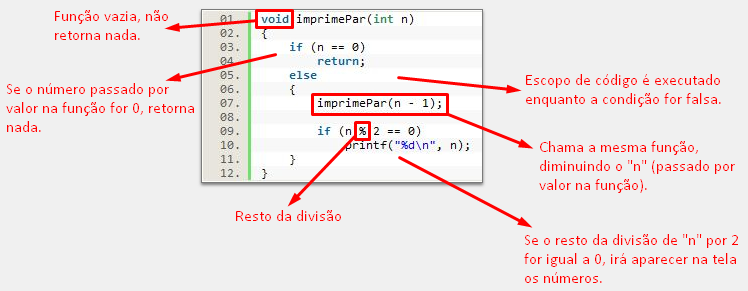
\includegraphics[scale=0.8]{Figuras/rec-adapt.png}
      \caption{Exemplo de algoritmo de impressão de número divisíveis por 2 na tela - Adaptado por Igor Carmona. \cite{imagem1}}
        \label{fig:exemplo1}
    \end{figure}

Na figura acima, segue um exemplo de algoritmo recursivo em linguagem C. Vale lembrar que independente da linguagem este recurso pode ser implementado basta seguir a sintaxe de cada linguagem.

\subsection{\textbf{Como utilizar a Recursão}}
\label{subsec:utilização}

Assim como já foi dito, um algoritmo recursivo pode ser utilizado quando queremos a solução de um grande problema. Para saber a direção certa da construção do seu algoritmo deve-se pensar em duas coisas: 

\subsection{\textbf{Cuidados a se tomar na Recursividade}}
\label{subsec:cuidados}

    \begin{itemize}
        \item O seu algoritmo deve ter \textbf{uma condição de parada}, isso porque conforme as chamadas da função forem sido executadas elas são empilhadas na memória do computador até que um valor é retornado para a \textit{main} e se caso não haja uma condição de pausa, você pode estourar a pilha de memória fazendo com que seu programa não execute mais.
        Após o retorno do valor pela função, o computador irá desempilhar as chamadas das funções e retornará o valor para cada valor chamado, resultando num valor total.
        \item Você deve padronizar o seu problema para uma forma genérica, um exemplo seria o fatorial de um número.
        
            %% Figura 2 %%
            \begin{figure}[H]
             \centering
             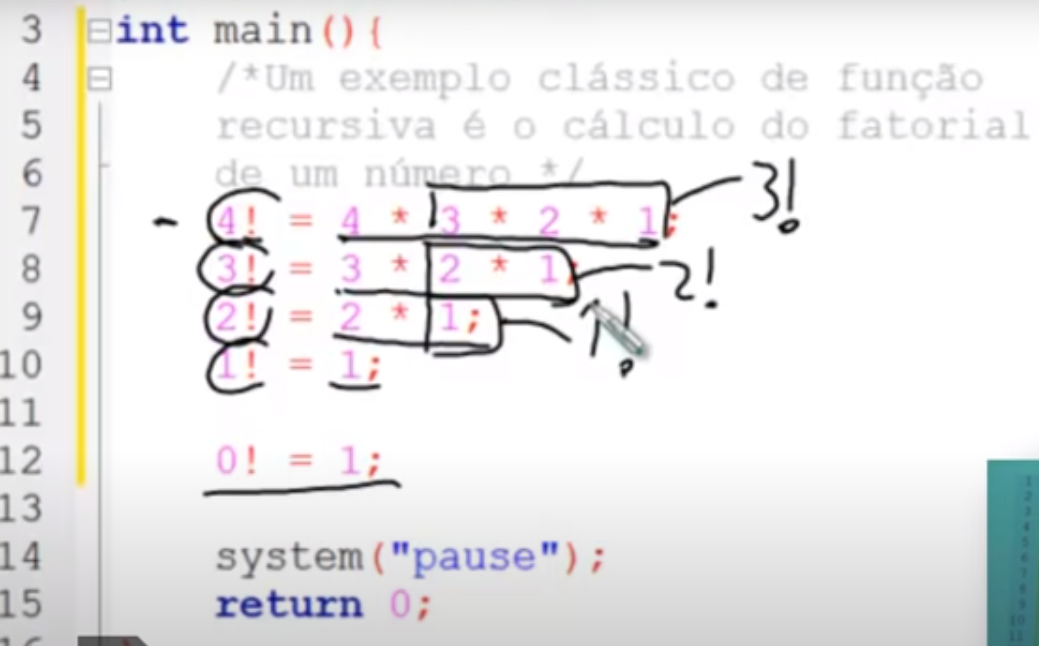
\includegraphics[scale=0.5]{Figuras/rec-fatorial.png}
             \caption{Exemplo de forma genérica para um código de recursão de um fatorial \cite{imagem2}}
             \label{fig:partições}
            \end{figure}
            
        Na imagem acima, temos um \textbf{caso base e a forma genérica} para montar um algoritmo recursivo. Observa-se que o fatorial de 4 é: 4 x \textbf{fatorial de 3}, enquanto é chamado a função passando \textbf{"n - 1"} temos: 3 x \textbf{fatorial de 2}, e assim por diante até chegar no \textbf{caso base} de \textbf{fatorial de 0} e \textbf{retornar um valor} e a partir disso começar o \textbf{processo de desempilhamento de memória}.
        
           %% Figura 3 %%
           \begin{figure}[H]
             \centering
             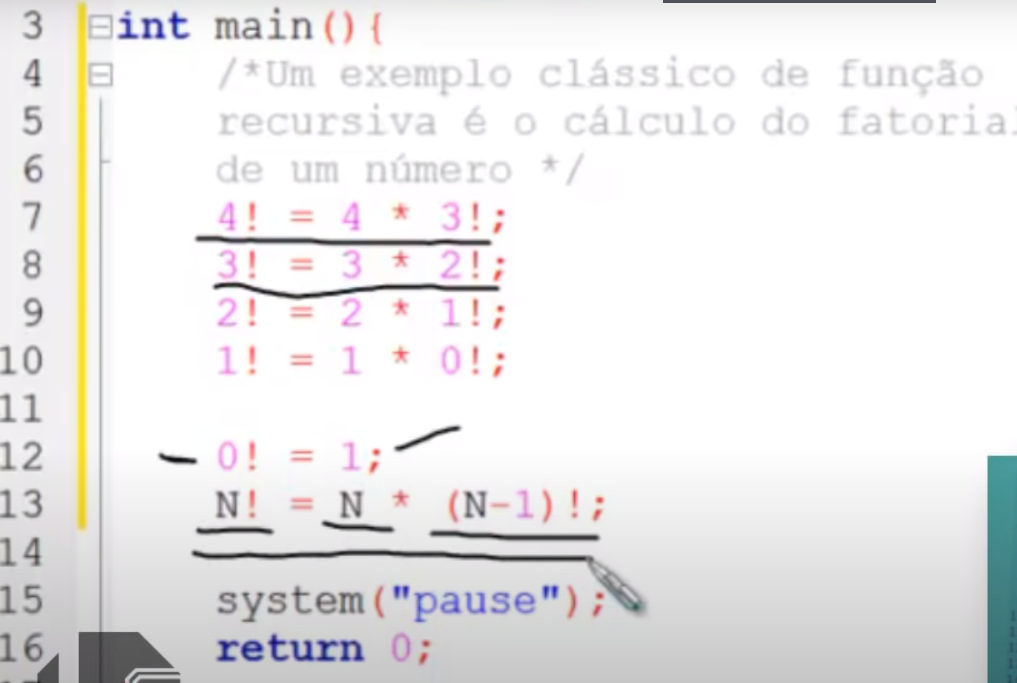
\includegraphics[scale=0.5]{Figuras/rec-fatorial2.png}
             \caption{Exemplo de forma genérica fatorial \cite{imagem3}}
             \label{fig:partições}
            \end{figure}
            
         \end{itemize}

\section{\textbf{Fundamentação de Árvore Binária}}
\label{sec:fundamentacao}

\subsection{\textbf{Compreensão de Nomenclaturas de Árvore comum}}
\label{subsec:árvore-comum}

Para um melhor entendimento sobre o tipo de árvore binária, recomenda-se ter conhecimento sobre as propriedades básicas de uma árvore comum e seu conceito que estão mutuamente interligadas com a recursão. Algumas nomenclaturas frequentemente utilizadas:

\begin{itemize}
    \subsubsection{\textbf{Nomenclaturas}}
    \item \textbf{VÉRTICES}: É cada uma das entidades representadas na árvore. Numa árvore, os vértices são classificados em \textbf{níveis}, sendo o número de nós no caminho entre o \textbf{vértice e a raiz}.
    \item \textbf{ARESTAS}: É uma conexão entre dois vértices.
    \item \textbf{PAI}: É o antecessor imediato de um vértice.
    \item \textbf{FILHO}: É o sucessor imediato de um vértice. Dado um determinado vértice, cada \textbf{filho} seu é a \textbf{raiz} de uma nova \textbf{sub-árvore}.
    \item \textbf{RAIZ}: É o vértice que não possui \textbf{pai}.
    \item \textbf{FOLHAS}: Qualquer vértice que não possui filhos. A raiz até uma de suas folhas denomina-se \textbf{altura da árvore}.
    \subsubsection{\textbf{Exemplos de uso na Computação}}
    \item Estrutura de diretórios (pastas).
    \item Busca de dados armazenados no computador.
    \item Representação de espaço de soluções como em um jogo de xadrez.
    \item Modelagem de algoritmos.
\end{itemize}

\subsection{\textbf{Conceitos sobre Árvore Binária, Árvore Estritamente Binária, Árvore Estritamente Binária completa}}
\label{subsec:conceitos}

\subsubsection{\textbf{Árvore Binária}}
\label{subsubsec:árvore-binária}

A árvore binária pode-se dizer que é um tipo especial de árvore, onde: 

\begin{itemize}
    \item Cada vértice pode ter duas sub-árvores sendo uma \textbf{sub-árvore esquerda} e a outra \textbf{sub-árvore direita}.
    \item O grau de cada um de seus vértices (número de filhos) pode ser \textbf{0, 1 ou 2} e sempre sua capacidade máxima será de 2 filhos.
\end{itemize}

\begin{figure}[H]
 \centering
     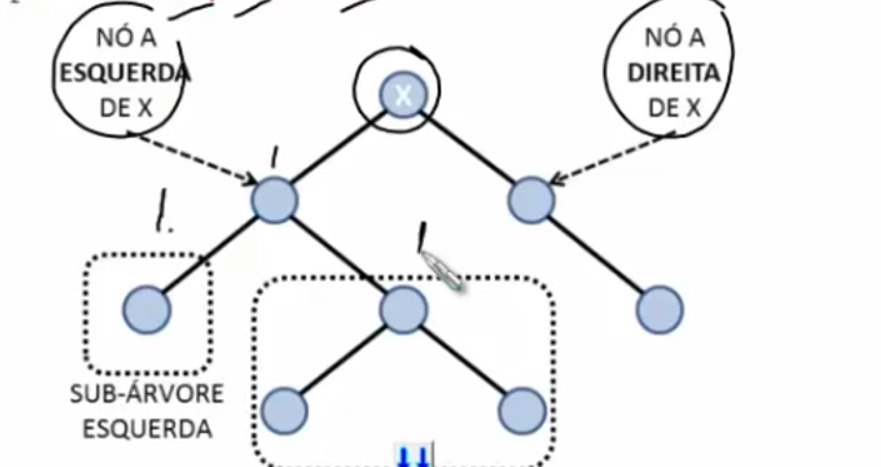
\includegraphics[scale=0.8]{Figuras/fig-binaria.png}
     \caption{Exemplo: representação em grafos da definição de árvore binária \cite{imagem4}}
    \label{fig:binaria}
 \end{figure}

\subsubsection{\textbf{Árvore Estritamente Binária}}
\label{subsubsec:estritamente-binária}

Temos também, a \textbf{Árvore Estritamente Binária} onde: 

\begin{itemize}
    \item Cada nó (vértice) possui \textbf{0 ou 2 sub-árvores}.
    \item Nenhum nó tem \textbf{filho único}.
    \item Nós internos (não folhas) sempre têm 2 filhos.
\end{itemize}

\begin{figure}[H]
 \centering
     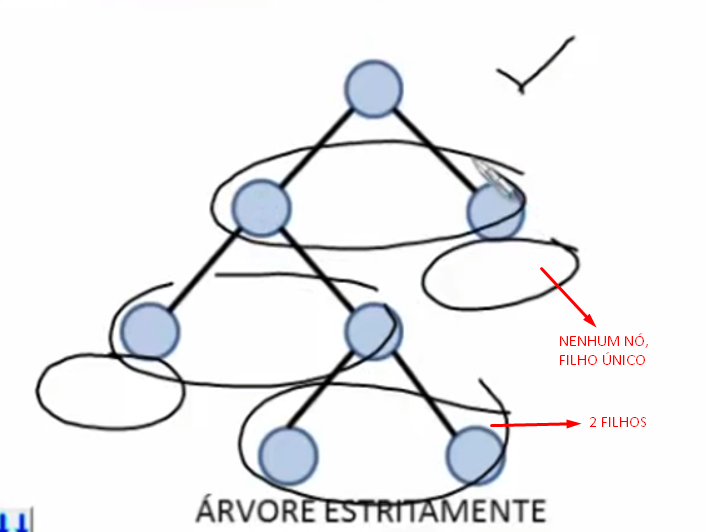
\includegraphics[scale=0.8]{Figuras/fig-estrita.png}
     \caption{Exemplo: representação em grafos de árvore estritamente binária \cite{imagem5}}
    \label{fig:estritamente-binária}
 \end{figure}

\subsubsection{\textbf{Árvore Binária Completa}}
\label{subsubsec:binária-completa}

\begin{figure}[H]
 \centering
     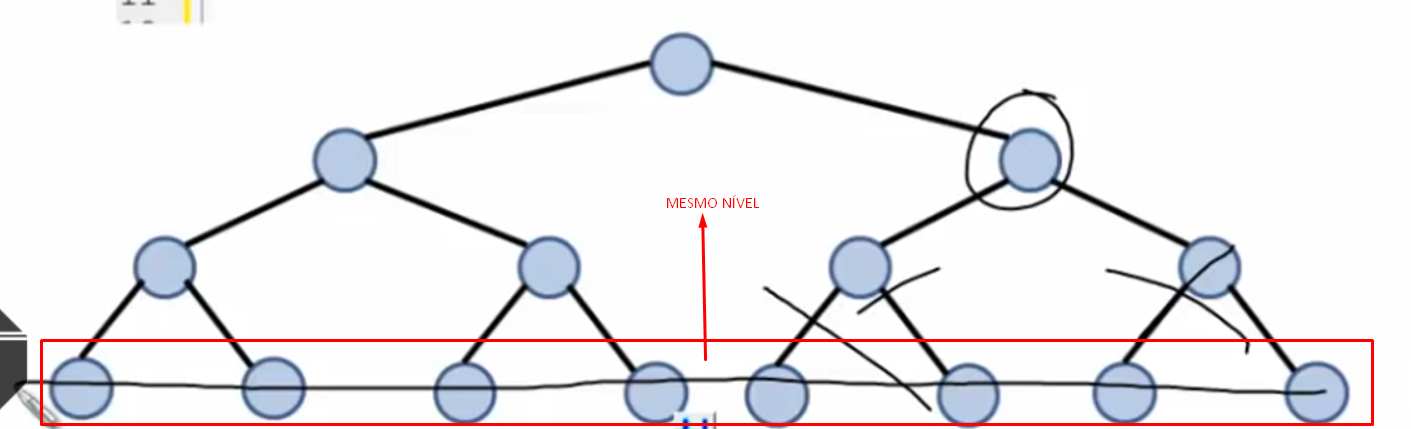
\includegraphics[scale=0.4]{Figuras/fig-quase.png}
     \caption{Exemplo: representação em grafos de árvore binária completa \cite{imagem6}}
    \label{fig:binaria-completa}
 \end{figure}

Na árvore binária completa tem um diferencial que é você poder fazer o cálculo do número de nós, na qual a fórmula matemática é $2^h^-^1$, sendo \textbf{"h"} a altura da árvore.

\begin{itemize}
    \item É estritamente binária.
    \item Todos os seus \textbf{nós-folha} estão no mesmo nível.
\end{itemize}

\section{\textbf{Conclusão}}
\label{sec:conclusao}

Há diversos outros tipos de árvores e aplicações de recursão para serem demonstradas mas a didática deste trabalho em si é apresentar conceitos, exemplificar e mostrar um novo mundo a se explorar. 

Vale lembrar, que foram dissertados assuntos relacionados a teoria de recursão e de árvores como uma forma de abrir o seu "mind-set". A complexidade na construção de algoritmos referente a esses temas foram abstratas para uma melhor compreensão dos iniciantes à programação.

\newpage
% ----------------------------------------------------------
% ELEMENTOS PÓS-TEXTUAIS
% ----------------------------------------------------------
\postextual
% ----------------------------------------------------------
% Referências bibliográficas
% ----------------------------------------------------------
\renewcommand{\bibsection}{%
\section{\bibname}
\bibmark
%\ifnobibintoc\else
%\phantomsection
%\addcontentsline{toc}{section}{\bibname}
%\fi
\prebibhook}

\bibliography{abntex2-modelo-references}

% ----------------------------------------------------------
% Apêndices
% ----------------------------------------------------------

% ---
% Inicia os apêndices
% ---
% \begin{apendicesenv}

% % ----------------------------------------------------------
% \section*{Apêndice A - Nome do Apêndice}
% \addcontentsline{toc}{section}{Apêndice A - Nome do Apêndice}
% % ----------------------------------------------------------

% \end{apendicesenv}
% % ---


% ----------------------------------------------------------
% Anexos
% ----------------------------------------------------------

% % ---
% % Inicia os anexos
% % ---
% \begin{anexosenv}

% % ---
% \section*{Anexo A - Nome do Anexo}
% \addcontentsline{toc}{section}{Anexo A - Nome do Anexo}
% % ---
% \end{anexosenv}


\end{document}
